% Reporte técnico — Barrel Ascent (formato Springer LNCS)
% Compilar: tectonic Reporte_Tecnico_BarrelAscent.tex
\documentclass[runningheads]{llncs}
\usepackage{fontspec}
\usepackage[spanish,es-noshorthands,es-tabla]{babel}
\usepackage{graphicx}
\usepackage{booktabs}
\usepackage{tabularx}
\usepackage{xcolor}
\usepackage{listings}
\usepackage{tikz}
\usetikzlibrary{arrows.meta,positioning,fit}
\usepackage{float}
\usepackage[hidelinks]{hyperref}

% ---- Datos del alumno (editar aquí) ----
\newcommand{\alumno}{Ashley Peña Nolasco}
\newcommand{\matricula}{178226}
% ----------------------------------------

\lstdefinestyle{cs}{language=[Sharp]C, basicstyle=\ttfamily\scriptsize, keywordstyle=\bfseries\color{blue!60!black},
  commentstyle=\itshape\color{gray}, stringstyle=\color{red!50!black}, frame=lines, framesep=2pt,
  xleftmargin=4pt, columns=fullflexible, showstringspaces=false, aboveskip=6pt, belowskip=4pt}
\lstset{style=cs}
\setlength{\emergencystretch}{1.5em}

\begin{document}

\title{Barrel Ascent: prototipo de plataformas 2D vertical en Unity}
\subtitle{Reporte técnico --- Laboratorio de Videojuegos (crédito por examen)}
\titlerunning{Barrel Ascent: reporte técnico}
\author{\alumno}
\authorrunning{\alumno}
\institute{Laboratorio de Videojuegos, Crédito por examen\\ ID: \matricula}

\maketitle

\begin{abstract}
Se presenta \emph{Barrel Ascent}, un juego de plataformas 2D en pixel art desarrollado en Unity~6 con
C\#. El jugador asciende por una fábrica de tres zonas mientras barriles autónomos ruedan y caen en zigzag.
El reporte describe la arquitectura por componentes comunicados mediante eventos, el renderizado con
cámara ortográfica \emph{pixel perfect} y seguimiento vertical suavizado, la física 2D con consultas
espaciales para suelo, escaleras y pisotón, y la inteligencia artificial de los barriles como máquina de
estados finitos con sensores. El prototipo se valida con 45 pruebas automáticas (PlayMode y EditMode) y
se entrega como ejecutable de macOS.
\keywords{Videojuegos \and Unity \and Plataformas 2D \and Máquina de estados \and Física 2D}
\end{abstract}

\section{Resumen del videojuego y objetivo}
\emph{Barrel Ascent} es una partida de 3--5 minutos en un único nivel vertical de $20\times46$ tiles. El
jugador se mueve, salta y escala para llegar a la baliza de la cima; recoge 10 piezas ($+100$), puede
destruir barriles cayendo sobre ellos ($+50$) y recibe $+250$ por cada zona superada y $+1000$ por la
meta. Tiene 3 vidas: un golpe lateral de barril o una caída fuera del nivel restan una. La partida tiene
los estados \emph{menú}, \emph{juego activo}, \emph{pausa}, \emph{victoria} y \emph{derrota}. El
diseño completo (reglas, controles y escenas) se describe en el documento de diseño (GDD).

El objetivo del proyecto es demostrar, en un prototipo acotado pero completo, los componentes
fundamentales de un videojuego vistos en el curso: renderizado y cámara, física e interacción,
inteligencia artificial, narrativa y una arquitectura de código explicable y comprobable.

\section{Relación con las bases del curso}
El juego pertenece al género de \textbf{plataformas arcade}, consolidado a inicios de los ochenta con
títulos como \emph{Donkey Kong}~\cite{dk,kent}, que estableció la estructura de vigas inclinadas,
escaleras y obstáculos que descienden mientras el personaje asciende. De esa tradición se conservan la
lectura inmediata de la pantalla, las reglas simples y el riesgo/recompensa de esquivar o enfrentar al
obstáculo. Se incorporan convenciones posteriores del género: desplazamiento de cámara (el nivel
mide cuatro pantallas de alto), dificultad progresiva por zonas y ayudas de \emph{game feel} como
\emph{coyote time} y \emph{jump buffer}, que hacen que el control se perciba justo~\cite{swink}.
La premisa (una línea de producción descontrolada que expulsa barriles desde la azotea) justifica el
recorrido vertical, el origen de los obstáculos y la meta visible.

\begin{figure}[H]
\centering
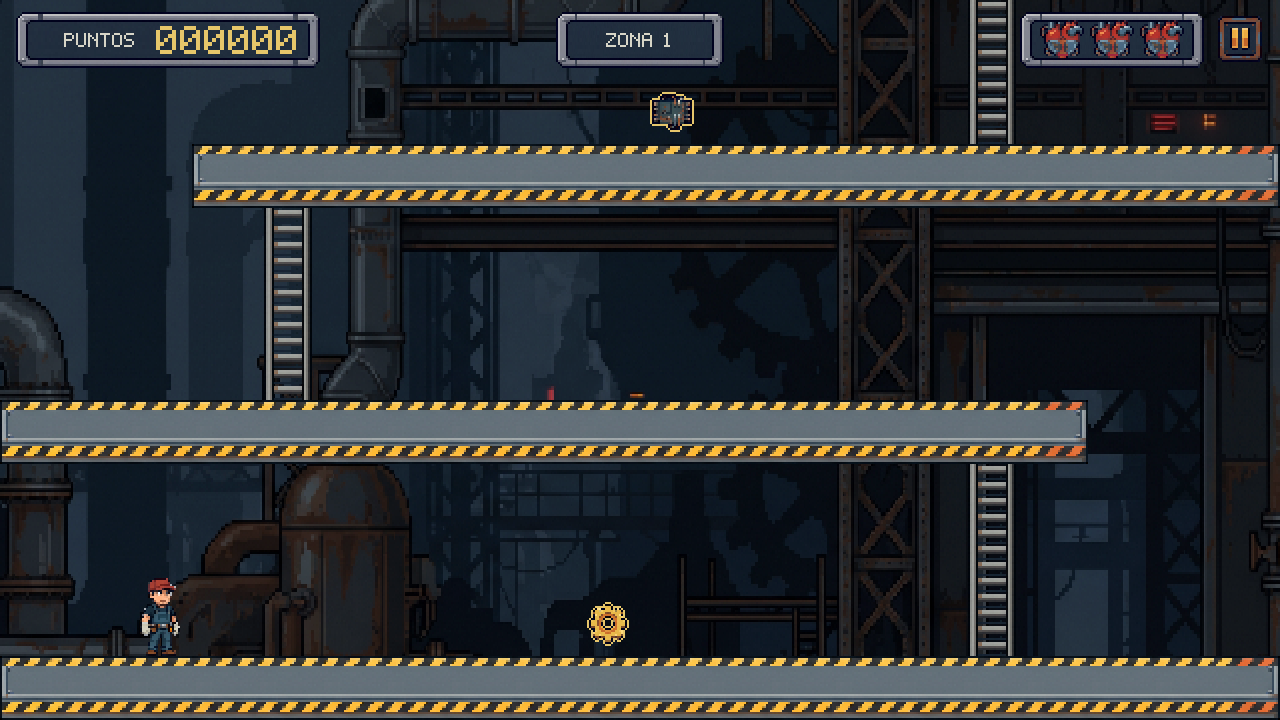
\includegraphics[width=\linewidth]{figs/UI_HUD.png}
\caption{Juego activo en la zona 1: HUD con puntuación, zona y vidas; vigas y escaleras del
Tilemap, un coleccionable y la técnica de mantenimiento controlada por el jugador.}\label{fig:juego}
\end{figure}

\section{Arquitectura general y organización del código}
El código (1\,993 líneas en 16 scripts, ensamblado \texttt{BarrelAscent}) se organiza por dominio:
\texttt{Player}, \texttt{Enemies}, \texttt{Environment}, \texttt{Managers}, \texttt{UI} y
\texttt{Effects}. Cada script es un \texttt{MonoBehaviour} con una única responsabilidad
(Fig.~\ref{fig:arq}). Dos gestores coordinan la partida: \texttt{GameManager} (estado, vidas,
puntuación, pausa y reinicio) y \texttt{LevelManager} (zona actual, bonus, reaparición y meta).

La comunicación sigue el patrón \emph{Observer}~\cite{nystrom}: los sistemas de juego
\emph{notifican} con eventos de C\# (\texttt{ScoreChanged}, \texttt{LivesChanged},
\texttt{StateChanged}, \texttt{ZoneChanged}, \texttt{Damaged}, \texttt{BarrelSmashed}, \ldots) y la
interfaz, los efectos y el audio solo \emph{escuchan}. Ningún script de juego conoce la UI, por lo que
\texttt{UIManager}, \texttt{EffectsManager} y \texttt{AudioManager} pueden quitarse sin romper las
reglas. Los datos de balance por zona viven en un \texttt{ScriptableObject} (\texttt{ZoneConfig}) y
se ajustan sin tocar código.

Una decisión de organización importante es que las escenas, prefabs y animaciones se construyen con
\textbf{constructores de editor reejecutables} (scripts \texttt{Phase\emph{N}Builder} en la carpeta
\texttt{Editor}): el nivel se
genera a partir de un archivo de texto (\texttt{LevelLayout.txt}, un carácter por tile) que el
constructor valida (escaleras apoyadas, marcadores presentes) antes de crear el Tilemap. Así el
proyecto es reproducible y cada cambio de diseño queda versionado como texto en git.

\begin{figure}[H]
\centering
\resizebox{\linewidth}{!}{\begin{tikzpicture}[>=Stealth, font=\scriptsize,
  b/.style={draw, rounded corners=2pt, fill=#1, minimum width=23mm, minimum height=5.5mm, align=center},
  b/.default=gray!10, l/.style={font=\tiny, fill=white, inner sep=1pt}]
\node[b=blue!10] (pc) at (0,0) {PlayerController};
\node[b=blue!10] (pcol) at (0,-0.85) {PlayerCollision};
\node[b=green!12] (col) at (0,-1.7) {Collectible / Goal};
\node[b=orange!15] (bs) at (0,-2.75) {BarrelSpawner};
\node[b=orange!15] (bc) at (0,-3.6) {BarrelController};
\node[b=red!10, minimum height=8mm] (gm) at (5.2,-0.85) {GameManager\\[-1pt]\tiny estado, vidas, puntos};
\node[b=red!10, minimum height=8mm] (lm) at (5.2,-2.75) {LevelManager\\[-1pt]\tiny zonas, bonus, meta};
\node[b] (ui) at (9.7,-0.1) {UIManager};
\node[b] (fx) at (9.7,-0.85) {EffectsManager};
\node[b] (au) at (9.7,-1.6) {AudioManager};
\node[b] (cam) at (9.7,-2.75) {CameraFollow};
\draw[->] (gm.north) |- node[l,above,pos=0.75]{SetControlEnabled} (pc.east);
\draw[->] (pcol) -- node[l,above]{Damaged / BarrelSmashed} (gm);
\draw[->] (col.east) -- node[l,above,sloped]{AddScore / ReachGoal} (lm.west);
\draw[->] (lm) -- node[l,right]{Win / AddScore} (gm);
\draw[->] (lm.south west) -- node[l,below,sloped]{activa por zona} (bs.east);
\draw[->] (bs) -- node[l,right]{instancia} (bc);
\draw[->, dashed] (gm.east) -- (ui.west);
\draw[->, dashed] (gm.east) -- (fx.west);
\draw[->, dashed] (gm.east) -- (au.west);
\draw[->] (lm) -- node[l,above]{SnapToTarget} (cam);
\node[draw=gray, dashed, fit=(ui)(fx)(au), inner sep=3pt, label={[font=\tiny]above:observadores (eventos)}] {};
\end{tikzpicture}}
\caption{Arquitectura. Flechas continuas: llamadas o eventos de juego; discontinuas: eventos que la
presentación escucha (la UI, los efectos y el audio también escuchan a jugador, barriles y zonas).}
\label{fig:arq}
\end{figure}

\section{Renderizado y cámara}
Se usa el \emph{Built-in Render Pipeline} con una cámara \textbf{ortográfica}, adecuada para 2D porque
no hay perspectiva: el tamaño ortográfico define cuántas unidades de mundo caben en pantalla. La
resolución de referencia es $640\times360$ con 32 píxeles por unidad (1 tile = 1 unidad), lo que da
$20\times11{,}25$ tiles visibles y un escalado entero $\times3$ en 1080p. El componente
\emph{Pixel Perfect Camera} garantiza ese escalado entero, y todas las texturas usan filtro
\emph{Point}, sin compresión ni \emph{mipmaps}, para que los píxeles no se difuminen.

La escena se dibuja por capas de ordenación (\emph{sorting order}): fondos por zona ($-20$), Tilemap de
vigas con su \texttt{TilemapRenderer}, escaleras, coleccionables, barriles y el jugador (10), y por
encima un \emph{Canvas} en \emph{Screen Space Overlay} para el HUD. Los tiles de viga se eligen
según sus vecinos (extremo izquierdo, tramo o extremo derecho). La animación del personaje es una
máquina de estados de \texttt{Animator} (Idle, Run, Jump con \emph{blend} por velocidad vertical,
Climb y Hurt) alimentada por parámetros que el controlador actualiza cada fotograma.

\texttt{CameraFollow} sigue al jugador solo en vertical (Listado~\ref{lst:cam}). Se ejecuta en
\texttt{LateUpdate}, después de que el jugador se haya movido; suaviza la altura con
\texttt{SmoothDamp}, la limita para no mostrar nada fuera del nivel y redondea solo la posición
\emph{final} a la rejilla de píxeles para evitar temblores.

El arte original (generado con Gemini a alta resolución) se procesa en el editor con \texttt{SpriteExtractor}:
elimina el fondo, separa fotogramas, alinea la cabeza del personaje al pivote para que no ``baile'' y
reduce cada sprite a la escala de 32\,PPU.

\par\noindent\begin{minipage}{\linewidth}
\begin{lstlisting}[caption={Actualización de la cámara (\texttt{CameraFollow.cs}).},label=lst:cam]
void LateUpdate() {
    float desired = ClampY(target.position.y + lookAheadY);
    // Se suaviza una Y sin redondear; solo la posición final se ajusta a píxel.
    smoothedY = ClampY(Mathf.SmoothDamp(smoothedY, desired, ref velocityY, smoothTime));
    SetPosition(smoothedY);          // redondea a 1/32 de unidad y fija X al centro
}
\end{lstlisting}
\end{minipage}\par

\section{Física, colisiones e interacciones}
La física usa el motor 2D de Unity (Box2D)~\cite{unity}. El jugador y los barriles son
\texttt{Rigidbody2D} dinámicos (gravedad $\times3$, rotación bloqueada, interpolación y detección
continua). Las vigas forman un único \texttt{CompositeCollider2D} generado desde el Tilemap, lo que
evita que el jugador se enganche en las juntas entre tiles. El movimiento se aplica en
\texttt{FixedUpdate} (paso fijo de física) y la lectura de entrada en \texttt{Update}.

\textbf{Capas y matriz de colisiones.} Se definen las capas \emph{Ground}, \emph{Ladder},
\emph{Player} y \emph{Barrel}. Los barriles ignoran a otros barriles, al jugador y a las escaleras en
la matriz de colisiones: así no empujan al jugador ni se atascan entre sí, y el contacto
jugador--barril se resuelve por código.

\textbf{Consultas espaciales.} En lugar de depender de los eventos de contacto, los sistemas preguntan
al mundo físico~\cite{ericson}: el jugador está en el suelo si un \texttt{OverlapBox} bajo sus pies toca
\emph{Ground}; el salto se acepta si el último contacto fue hace $\le0{,}08$\,s (\emph{coyote time}) y
la pulsación hace $\le0{,}1$\,s (\emph{jump buffer}). Al escalar, la gravedad pasa a 0 y
\texttt{Rigidbody2D.excludeLayers} permite atravesar la viga superior hasta quedar de pie sobre ella.
El Listado~\ref{lst:jump} muestra cómo se combinan ambas tolerancias y cómo se consume el contacto
para impedir el doble salto.

\textbf{Jugador--barril.} Cada paso físico \texttt{PlayerCollision} obtiene los barriles que se solapan
con su cápsula. Si los pies están por encima del centro del barril (con un margen de 0,05\,u) y la
velocidad vertical del jugador no supera 2\,u/s, es un
\emph{pisotón}: el barril se destruye y el jugador rebota a 9\,u/s. En otro caso es un \emph{golpe
lateral}: retroceso, $-1$ vida y 1,5\,s de invulnerabilidad con parpadeo. Coleccionables, meta y
zonas usan \emph{triggers}; cada coleccionable desactiva su collider al recogerse para puntuar una
sola vez.

\begin{table}[H]
\caption{Parámetros físicos principales (ajustables en el inspector).}\label{tab:fis}
\centering\scriptsize
\begin{tabularx}{\linewidth}{@{}lX@{}}
\toprule
\textbf{Elemento} & \textbf{Valores} \\ \midrule
Jugador & Cápsula $0{,}6\times0{,}94$\,u; velocidad 5\,u/s; impulso de salto 10\,u/s; gravedad $\times3$; escalada 3\,u/s \\
Ayudas de salto & \emph{Coyote time} 0,08\,s; \emph{jump buffer} 0,1\,s \\
Daño y pisotón & Retroceso $(3,5)$\,u/s con 0,25\,s sin control; invulnerabilidad 1,5\,s; rebote 9\,u/s \\
Barril & Círculo $r=0{,}4$\,u; 2 / 2,75 / 3,5\,u/s según zona; en caída conserva el 50\,\% de la velocidad horizontal \\
Nivel & Límite de caída $y=-3$; capas Ground, Ladder, Player, Barrel \\
\bottomrule
\end{tabularx}
\end{table}

\par\noindent\begin{minipage}{\linewidth}
\begin{lstlisting}[caption={Salto con \emph{coyote time} y \emph{jump buffer} (\texttt{PlayerController.cs}).},label=lst:jump]
void TryJump() {
    bool requested = Time.time - jumpRequestTime <= jumpBufferTime;
    bool canJump   = Time.time - lastGroundedTime <= coyoteTime;
    if (!requested || !canJump) return;
    body.linearVelocity = new Vector2(body.linearVelocity.x, jumpForce);
    jumpRequestTime  = float.NegativeInfinity;
    lastGroundedTime = float.NegativeInfinity;   // consume el contacto: sin doble salto
    Jumped?.Invoke();                            // evento para efectos y audio
}
\end{lstlisting}
\end{minipage}\par

\section{Inteligencia artificial: barriles autónomos}
Cada barril es un agente reactivo modelado como \textbf{máquina de estados finitos}~\cite{millington}
(Fig.~\ref{fig:fsm}), evaluada en \texttt{FixedUpdate} (Listado~\ref{lst:fsm}). Percibe su entorno con
dos sensores sobre la capa \emph{Ground}: un \texttt{OverlapBox} estrecho bajo su centro (¿hay suelo?)
y un \texttt{Raycast} horizontal de 0,06\,u desde su borde (¿hay pared?).

El comportamiento emergente es el descenso en zigzag: como las vigas tienen un extremo abierto
alterno, cada barril recorre una viga, cae a la inferior y sigue en sentido opuesto, cruzando la ruta del
jugador en cada piso. Se añaden salvaguardas para que ningún agente quede ``vivo'' indefinidamente:
detección de atasco (sin avance durante 1\,s), límite inferior y vida máxima de 90\,s.

La decisión de \emph{cuándo} atacar la toma un segundo nivel: cada zona tiene un
\texttt{BarrelSpawner} que lanza barriles con el intervalo y la velocidad de su \texttt{ZoneConfig}
(4\,s y 2\,u/s; 3\,s y 2,75\,u/s; 2\,s y 3,5\,u/s; máximo 6 vivos), y el \texttt{LevelManager} activa
solo el generador de la zona donde está el jugador. La dificultad responde así a su progreso.

\begin{figure}[H]
\centering
\begin{tikzpicture}[>=Stealth, font=\scriptsize,
  s/.style={draw, rounded corners=3pt, fill=orange!12, minimum width=19mm, minimum height=6mm},
  l/.style={font=\tiny, align=center}]
\node[s] (sp) at (0,0) {SPAWNED};
\node[s] (ro) at (3.9,0) {ROLLING};
\node[s] (fa) at (7.8,0) {FALLING};
\node[s, fill=gray!15] (de) at (3.9,-2) {DESTROYED};
\draw[->] (sp) -- node[l,above]{0,3\,s y apoyado} (ro);
\draw[->] (ro.20) -- node[l,above]{sin suelo bajo el centro} (fa.160);
\draw[->] (fa.200) -- node[l,below]{aterriza: invierte el sentido} (ro.340);
\draw[->] (ro) -- node[l,right,pos=0.55]{pared delante, atasco 1\,s\\ o pisotón del jugador} (de);
\draw[->] (fa) |- node[l,pos=0.3,right]{pisotón o\\bajo el nivel} (de);
\draw[->] (sp) |- node[l,pos=0.3,left]{vida\\máx. 90\,s} (de);
\end{tikzpicture}
\caption{Máquina de estados del barril.}\label{fig:fsm}
\end{figure}

\par\noindent\begin{minipage}{\linewidth}
\begin{lstlisting}[caption={Núcleo de la máquina de estados (\texttt{BarrelController.cs}).},label=lst:fsm]
switch (CurrentState) {
  case State.Rolling:
    if (!grounded)      { EnterState(State.Falling); break; } // fin de la viga
    if (IsWallAhead())  { Despawn(); break; }                 // fin del recorrido
    body.linearVelocity = new Vector2(direction * speed, body.linearVelocity.y);
    break;
  case State.Falling:
    body.linearVelocity = new Vector2(direction * speed * 0.5f, body.linearVelocity.y);
    if (grounded && body.linearVelocity.y <= 0.01f) {
      direction = -direction; EnterState(State.Rolling);    // zigzag
    }
    break;
}
\end{lstlisting}
\end{minipage}\par

\section{Herramientas y lenguaje}
Se eligió \textbf{Unity 6 (6000.4) con C\#}, opción contemplada en el programa. Frente a
Three.js/WebGL u OpenGL con C++, Unity ofrece ya resueltos el bucle de juego, la física 2D, el sistema
de Tilemap, el \emph{Animator} y la UI, lo que permitió centrar el esfuerzo en los componentes que se
evalúan (cámara, reglas, IA) en lugar de en infraestructura~\cite{gregory}. C\# aporta tipado estático,
eventos nativos y una integración directa con el inspector. Se usaron los paquetes \emph{2D Tilemap},
\emph{2D Pixel Perfect}, \emph{Input System} (acciones de teclado declaradas en un asset), \emph{uGUI}
con \emph{TextMeshPro} y \emph{Unity Test Framework}; el control de versiones se llevó con git, con un
\emph{commit} por fase de desarrollo.

\textbf{Ejecución.} Abrir \texttt{Builds/macOS/Barrel Ascent.app} (la primera vez: clic derecho
$\rightarrow$ \emph{Abrir}, pues no está firmada con certificado de Apple). Para el código: abrir la
carpeta del proyecto en Unity 6000.4 y ejecutar la escena \texttt{MainMenu}.

\section{Pruebas, problemas encontrados y correcciones}
Las pruebas se automatizaron con \emph{Unity Test Framework}, simulando el teclado con el Input
System sobre las escenas reales (Tabla~\ref{tab:tests}). Las 45 pruebas pasan en la versión entregada.
Además se jugó manualmente cada fase y el ejecutable final se verificó arrancándolo sin el editor.

Problemas relevantes y su corrección:
\begin{itemize}
\item \textbf{Cámara atascada a altos FPS.} Al suavizar desde la posición ya redondeada a píxel, cada
paso era menor que medio píxel y la cámara no avanzaba. Se suaviza un valor sin redondear y solo se
redondea la posición final (Listado~\ref{lst:cam}).
\item \textbf{Jugador enganchado en las juntas de las vigas.} Un collider por tile producía aristas
internas; se sustituyó por un \texttt{CompositeCollider2D} combinado y un material sin fricción.
\item \textbf{Barril atascado en una esquina (zona 3).} Al caer chocaba con el borde de la viga
inferior; la prueba de recorrido lo detectó y se movió su punto de aparición una columna.
\item \textbf{Pruebas bloqueadas con el juego pausado.} Con \texttt{timeScale}\,=\,0 las esperas por
paso físico nunca terminan; los auxiliares de prueba fallan de inmediato en ese caso.
\item \textbf{Espacio pulsaba botones al reanudar.} El botón seleccionado seguía activo; la UI
deselecciona todo al volver al juego.
\item \textbf{Legibilidad.} El brillo del fondo de la zona 2 ocultaba barriles y un coleccionable oscuro
no se veía en la zona 3: se oscurecieron fondos y se añadió un contorno de 1\,px a los coleccionables.
\end{itemize}

\begin{table}[H]
\caption{Pruebas automáticas por conjunto.}\label{tab:tests}
\centering\scriptsize
\begin{tabularx}{\linewidth}{@{}lcX@{}}
\toprule
\textbf{Conjunto} & \textbf{N.} & \textbf{Qué comprueba} \\ \midrule
PlayerController & 5 & Movimiento, salto sin doble salto, escaleras, sin deriva. \\
GameLevel & 7 & Las 12 escaleras y los 5 saltos obligatorios; límites de cámara; zonas. \\
Barrel & 6 & Secuencia de estados, giro al aterrizar, pared, pisotón, daño único, spawner. \\
GameRules & 9 & Puntos, vidas, invulnerabilidad, caída, bonus, victoria, pausa, reinicio. \\
UI & 6 & Fuente, menú, HUD por eventos, paneles y navegación con teclado. \\
ArtAudio & 6 & Animaciones del jugador, efectos y sonido por evento. \\
Final & 2 & Sesión completa menú$\rightarrow$meta$\rightarrow$menú (×2) y resistencia de 60\,s. \\
EditMode & 4 & Escenas del build, sin placeholders, ajustes de texturas, Animator completo. \\
\midrule
\textbf{Total} & \textbf{45} & \\
\bottomrule
\end{tabularx}
\end{table}

\section{Limitaciones y mejoras futuras}
El prototipo tiene un solo nivel y se controla solo con teclado; no guarda récords ni opciones de
volumen. El ejecutable es solo para macOS y no está firmado ni notarizado. Algunas animaciones del
paquete de arte (bajar de espaldas, voltereta de daño) no se usan, y los MP3 pueden dejar un hueco
mínimo al repetir el bucle. Como mejoras se proponen: tabla de puntuaciones persistente, soporte de
mando, más niveles generados desde el mismo formato de texto, barriles con comportamientos
variados (por ejemplo, que bajen por escaleras con cierta probabilidad) y builds para Windows y Web.

\section{Conclusiones}
El proyecto evidencia los ejes del curso en un producto jugable: el \textbf{tipo de videojuego} y su
historia se reflejan en un plataformas arcade con premisa propia; el \textbf{renderizado} en la cámara
ortográfica \emph{pixel perfect}, el orden de capas y el seguimiento en \texttt{LateUpdate}; la
\textbf{física} en cuerpos rígidos, capas, \emph{triggers} y consultas espaciales; la \textbf{IA} en
una máquina de estados con sensores y un generador que adapta la dificultad; y la
\textbf{programación} en una arquitectura de componentes desacoplados por eventos, construida de
forma reproducible y validada con pruebas automáticas. La principal lección fue que pequeñas
decisiones técnicas (dónde redondear la cámara, cómo combinar colliders) determinan directamente la
sensación de juego.

\subsubsection*{Recursos de terceros.}
Motor y paquetes de Unity Technologies~\cite{unity}. Sprites, tileset, fondos y elementos de interfaz
creados por la autora con la IA generativa Gemini de Google~\cite{gemini} y procesados en el proyecto
(\texttt{SpriteExtractor}). Música y efectos de sonido obtenidos de Pixabay~\cite{pixabay}, bajo su
licencia de contenido gratuito (\texttt{Assets/Audio}). Fuente pixel generada por código.

\begin{thebibliography}{10}
\bibitem{dk} Nintendo: Donkey Kong. Videojuego arcade, Kioto (1981)
\bibitem{kent} Kent, S.L.: The Ultimate History of Video Games. Three Rivers Press, Nueva York (2001)
\bibitem{swink} Swink, S.: Game Feel: A Game Designer's Guide to Virtual Sensation. Morgan Kaufmann,
Burlington (2009)
\bibitem{nystrom} Nystrom, R.: Game Programming Patterns. Genever Benning (2014)
\bibitem{millington} Millington, I.: AI for Games, 3rd edn. CRC Press, Boca Raton (2019)
\bibitem{ericson} Ericson, C.: Real-Time Collision Detection. Morgan Kaufmann, San Francisco (2004)
\bibitem{gregory} Gregory, J.: Game Engine Architecture, 3rd edn. CRC Press, Boca Raton (2018)
\bibitem{unity} Unity Technologies: Unity 6 Manual, \url{https://docs.unity3d.com/Manual/}
\bibitem{gemini} Google: Gemini (IA generativa), \url{https://gemini.google.com}
\bibitem{pixabay} Pixabay: Música y efectos de sonido gratuitos, \url{https://pixabay.com}
\end{thebibliography}

\end{document}
